\chapter{Basic Notions - Nozioni Base}
\thispagestyle{chapterInit}
\section{The CIA Triad}
\label{sec:ciaTriad}
    \subsection{Introduzione}
    \paragraph{L'acronimo} L'acronimo CIA in inglese sta per \textbf{Confidentiality}, \textbf{Integrity} e \textbf{Availability}. Questi tre concetti sono alla base della sicurezza informatica e della protezione dei dati.  
        \subparagraph{Confidentiality - Riservatezza}
        \label{subPar:confidentiality}
            Il principio della Riservatezza prescrive che i non autorizzati non devono poter accedere ai dati e i dati sono visibili solo a chi è autorizzato a vederli.
        \subparagraph{Integrity - Integrità}
        \label{subPar:integrity}
            Il principio di Integrità prescrive che i dati non devono essere modificati se non da persone autorizzate a farlo, i tentativi di modifica non autorizzati devono essere rilevati e prevenuti.
        \subparagraph{Availability - Disponibilità}
            Il principio della Disponibilità prescrive che i dati non devono essere mantenuti inaccessibili ed inoltre bisogna permettere l'accesso agli autorizzati alle informazioni e ai servizi.
    \subsection{In Pratica}
        \paragraph{Confidentiality - Riservatezza}
            L'accesso alle informazioni riservare può essere:
            \subparagraph{Intenzionale} Quando un intruso cerca di accedere a dati sensibili.
            \subparagraph{Non Intenzionale} Quando un utente autorizzato accede a dati sensibili senza volerlo causato dal fatto che chi detiene i dati non è competente e/o non gli importa della sicurezza.
        
            Come garantire la riservatezza:
            \subparagraph{Crittografia} La \textbf{crittografia} è una tecnica che permette di limitare l'accesso ai dati solo a chi possiede la chiave per decifrarli (e quindi è autorizzato).
            \subparagraph{Access Control} Il \textbf{controllo degli accessi} è una parte integrante per mantenere la \textbf{riservatezza}, ciò andando a gestire quali utenti possono accedere a quali risorse.
        \paragraph{Integrity - Integrità}
            Per garantire l'integrità bisogna prevenire la modifica e/o la distruzione, inoltre bisogna assicurare informazioni autentiche e non invalidate.

            Inoltre ulteriore prescrizione è quella di individuare anche le cosiddette "minute changes" ovvero le modifiche minime che possono essere fatte ai dati per alterarne il significato. 
            
            L'integrità può essere anche di tipo \textbf{data integrity} ovvero la garanzia che i dati siano corretti e completi, oppure di tipo \textbf{system integrity} ovvero la garanzia che il sistema sia protetto da attacchi e che funzioni correttamente.

            L'itemize può essere compromessa da:
            \begin{itemize}
                \item errore umano
                \item attacchi come malware distruttivi e ransomware
            \end{itemize}
            Come garantire l'integrità:
            \subparagraph{Version Control} Il \textbf{controllo delle versioni} assieme agli \textbf{audit trails} permettono ad una organizzazione di garantire la veridicità dei dati.
            \subparagraph{Compliance requirements} I \textbf{requisiti di conformità} sono regole e normative che un'organizzazione deve seguire per garantire l'integrità dei dati.
        \paragraph{Availability - Disponibilità}
            Le violazioni alla disponibilità includono:
            \begin{itemize}
                \item Fallimento dell'infrastruttura 
                \item Overload dell'infrastruttura
                \item Blackout
                \item Attacchi come DDoS
            \end{itemize}
            Come garantire la disponibilità:
            \subparagraph{Backup} Bisogna sempre avere un piano di \textbf{backup} per mantenere disponibile in caso di disastro, attacco o altre minacce si verificassero.
            \subparagraph{Cloud} Il \textbf{cloud} è una soluzione per garantire la disponibilità dei dati, in quanto i dati sono replicati su più server e quindi in caso di guasto di uno di essi i dati sono comunque disponibili.
        
\section{Security Policy, Mechanism, Service}
    \subsection{Security Policy}
            \subsubsection{Definizione}
                Una \textbf{security policy} è un insieme di regole e requisiti stabilita da una azienda che definisce l'uso accettabile delle informazioni e dei servizi, inoltre il livello indica il livello di confidenzialità, integrità e disponibilità delle informazioni.
            \subsubsection{Esempi}
                Un esempio di possibili regole di una \textbf{security policy} potrebbero essere:
                \begin{itemize}
                    \item I dipendenti devono completare il corso su sicurezza informatica e accettare la policy di sicurezza.
                    \item I visitatori dell'azienda devono essere accompagnati da un dipendente autorizzato in tutti i momenti, questo dipendente deve mantenere i visitatori in una area appropriata senza dati sensibili
                    \item I dipendenti devono mantenere una "scrivania pulita" dunque senza lasciare documenti sensibili accessibili e incustoditi.
                    \item I dipendenti devono usare una password sicura e queste non devono essere usate in altri servizi esterni.
                    \item Gli ex-dipendenti non devono mantenere alcun dato dell'azienda.
                \end{itemize}
    \subsection{Security Service}
            \subsubsection{Definizione} La capacità di supportare uno o più dei requisiti di sicurezza (Confidentiality, Integrity, Availability) e.s.: gestione chiavi, controllo accessi, autenticazione.
                Come già detto i \textbf{Security Services} implementano uno o più \textbf{Security Mechanism} che servono per far rispettare la \textbf{Security Policy}.
            \subsubsection{Esempi}
                \paragraph{HTTP(S)}
                    \subparagraph{HTTP} Se si sua il protocolla \textbf{HTTP} per la trasmissione dei dati qualsiasi informazione trasmessa può venire intercettata da hacker nel mezzo.
                    \subparagraph{HTTPS} Per ovviare a questo problema si usa il protocollo \textbf{HTTPS} che è una versione sicura di \textbf{HTTP} che usa la crittografia per proteggere i dati, in questo modo i dati trasmessi vengono cifrati e se intercettati non possono essere letti.
                \paragraph{Access Control}
                    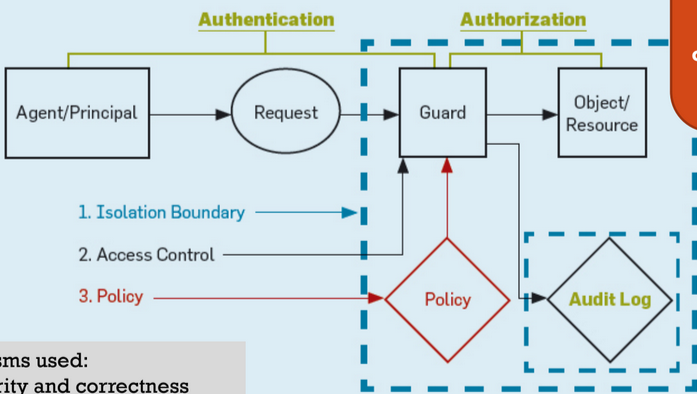
\includegraphics[height=12.5em]{01/accessControlSchema.png}
                    \subparagraph{Audit Log} è un registro importante che registra tutte le richieste di accesso ai dati e se la richiesta è stata accettata o rifiutata, in questo modo si può monitorare se una richiesta che è stata fatta ha avuto un risultato non aspettato e quindi che vadano modificate le \textbf{policy}.
    \subsection{Security Mechanism}
    \label{subsec:securityMechanism}
        \subsubsection{Definizione} Un \textbf{security mechanism} un dispositivo o funzione designato per provvedere uno o più servizi di sicurezza classificate in termini di potenza
            
            Inoltre è l'implementazione della \textbf{security policy}
        \subsubsection{Esempi}
    \subsection{Come si relazionano}
        In conclusione i \textbf{Security Services} implementano uno o più \textbf{Security Mechanism} che servono per far rispettare la \textbf{Security Policy}.
        
        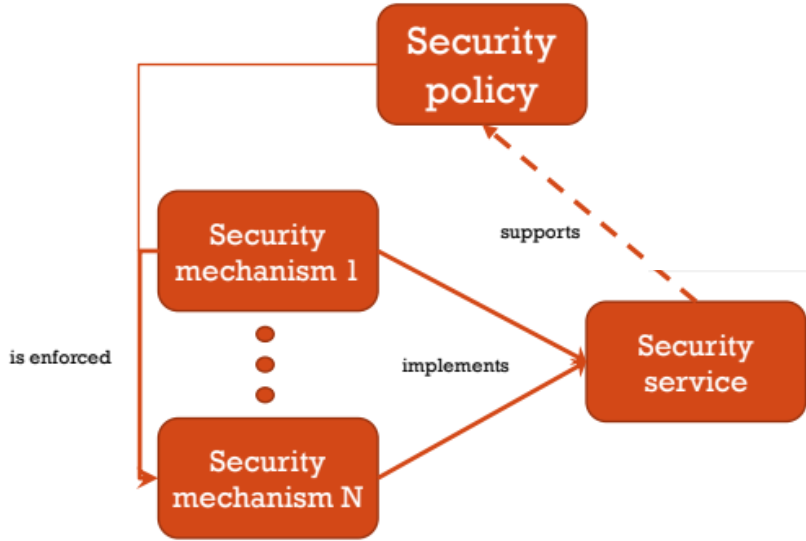
\includegraphics[height=10em]{01/schemaSecurity.png}
\section{CIA, Security Violation, and Mitigation}
    \paragraph{} La triade CIA non è solo essenziale per rendere sicuri i dati ma aiuta anche a capire cosa è andato storto nel caso di una \textbf{security violation}
    \subsection{Attacco Ransomware}
        \paragraph{L'arttacco}
            Nel caso di un attacco ransomware i dati vengono tenuti in ostaggio e la vittima viene ricattata con la pubblicazione di dati personali o il mancato accesso ad essi fino a che un riscatto non viene pagato.

            Questo attacco cripta i dati rendendoli inaccessibili e per ripristinarli è necessaria una chiave di decodifica, i pagamenti solitamente vengono eseguiti in crypto valute poco tracciabili.

            Questo genere di attacco viola la \textbf{confidentiality} e la \textbf{availability} dei dati.
        \paragraph{Mitigation}
            Per mitigare il rischio (che comunque non può essere eliminato) è utile procedere con un approccio \textbf{Zero Thrust} ovvero un "protocollo" che richiede che tutti gli utenti all'interno e all'esterno della rete aziendale siano autenticati e che la connessione è continuamente validata, prima di consentire accesso a applicazioni e dati.

\section{Risk}
    \paragraph{} Non esiste un sistema sicuro, esistono solo diversi livelli di insicurezza, si punta sempre ad ottenere il miglior livello di sicurezza possibile con il budget a disposizione.
    \subsection{Vulnerability}
        \subsubsection{Definizione}
            Una \textbf{vulnerabilità} è una debolezza in un sistema informativo, un sistema di sicurezza, nei controlli interni o nell'implementazione di questi. Questa debolezza può essere sfruttata o compromessa da una minaccia alla sicurezza.
        \subsubsection{Examples}
            Un esempio di \textbf{vulnerabilità} è una backdoor nascosta nel software e/o hardware, oppure dei bug non conosciuti di un software, o anche delle password deboli.
    \subsection{Threat}
        \subsubsection{Definizione}
            Qualunque circostanza o evento con il potenziale per causare perdite o danni a: operazioni dell'azienda, risorse o individui che possono accedere a tali risorse tramite un accesso non autorizzato, distruzione, pubblicazione, modifica e/o DoS. Inoltre un \textbf{threat} è un potenziale attacco che sfrutta una \textbf{vulnerabilità} del sistema.
        \subsubsection{Examples}
                Un esempio di \textbf{threat} sono:
                \begin{itemize}
                    \item Hacker:
                        \begin{itemize}
                            \item Trova e/o \textbf{sniff} una password.
                            \item Una il \textbf{social engineering} per ottenere informazioni sensibili e password.
                            \item Occupa le risorse di sistema con richieste inutili (attacchi DoS).
                        \end{itemize}
                    \item Virus e worms:
                        \begin{itemize}
                            \item I \textbf{virus} sono programmi auto replicanti che richiedono una azione dell'utente per essere attivati, esempio ne è una Email, un allegato o un link o un Floppy/CD/USB infetto.
                            \item I \textbf{worms} sono programmi auto replicanti che non richiedono una azione dell'utente per essere attivati, esempio ne è un worm che sfrutta una vulnerabilità di un sistema operativo.
                        \end{itemize} 
                \end{itemize}
    \subsection{Attack}
        \subsubsection{Definizione} Un \textbf{attacco} è un qualsiasi attività dannosa che prova a raccogliere, degradare, negare o distruggere informazioni o servizi. Può anche manifestarsi sotto un tentativo di ottenere un accesso ad una risorsa alla quale non si ha diritto 
    \subsection{Risk}
        \subsubsection{Definizione}
            Il \textbf{rischio} è la \textbf{probabilità} che una particolare \textbf{minaccia} \textbf{sfrutti} una particolare \textbf{vulnerabilità}.Il \textbf{rischio} è inoltre una misura di quanto una particolare circostanza o evento possa essere potenzialmente minacciato ed è tipicamente in funzione di: 
            \begin{enumerate}
                \item L'impatto che questa circostanza o evento potrebbe avere
                \item La probabilità che questa circostanza o evento si verifichi
            \end{enumerate}
        \subsubsection{Riassumendo}
            Riassumendo le \textbf{minacce} sono una combinazione di \textbf{intento} e \textbf{capability} di un attacco con successo. Invece le \textbf{vulnerabilità} sono caratterizzate da quanto è facile \textbf{identificarle} e \textbf{sfruttarle}.
            
            C'è da dire che l'impatto di un attacco deve essere valutato dal punto di vista di ogni soggetto coinvolto, ad esempio un attacco che compromette la privacy di un singolo individuo può avere un impatto molto diverso se lo si guarda dal punto di vista dell'individuo o dell'azienda.
        \subsubsection{Risk Matrix}
            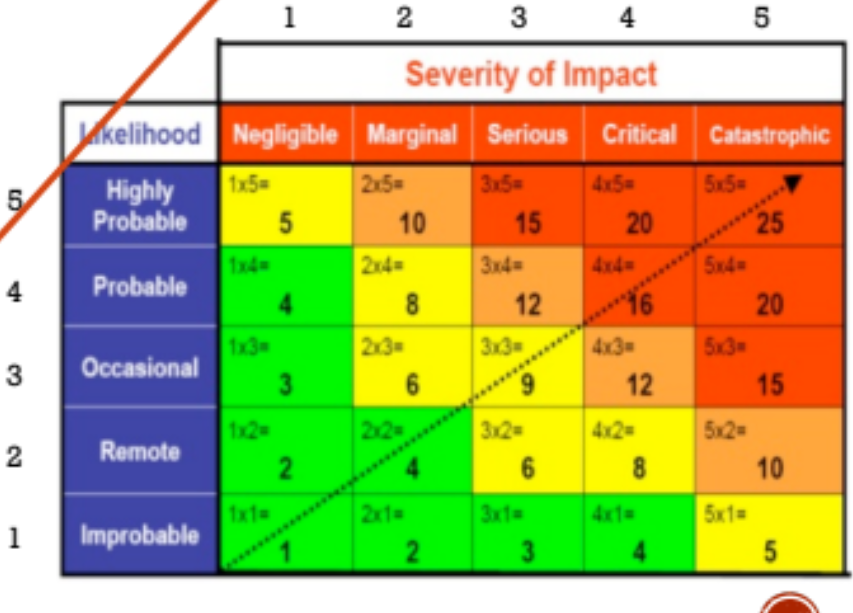
\includegraphics[height=10em]{01/riskMatrix.png}
            
            La presente matrice è una rappresentazione grafica del rischio, in cui si valuta la probabilità di un attacco e l'impatto che questo avrebbe, solitamente un rischio per essere accettabile deve avere un valore risultante tra basso (1-4) e medio-basso (5-9), i valori quali medio-alto (10-14) e alto (15-25) sono considerati inaccettabili e quindi devono essere mitigati abbassando la probabilità di attacco e/o l'impatto che questo avrebbe.

\section{Fine della diffusione degli attacchi}
    \paragraph{Generalmente} Il rischio è causato dunque dalla somma di una minaccia e una vulnerabilità, la minaccia è la capacità di sfruttare una vulnerabilità per causare un danno. 
    \paragraph{Pianizifazione} Quando si studiano i rischi sia prima che dopo un attacco bisogna considerare che se la \textbf{Minaccia - Threat} riesce a sfruttare la \textbf{Vulnerabilità - Vulnerability} allora si ha un \textbf{Rischio - Risk} se questo risulta inaccettabile allora si deve procedere con la \textbf{Mitigazione - Mitigation} del rischio, ciò riduce la \textbf{Minaccia - Threat} e il ciclo riprende fino a quando il \textbf{Rischio residuo - Residual Risk} è accettabile.

\section{Security \& Human Factor - Sicurezza \& Fattore Umano}
    Il fattore umano è uno dei fattori più importanti nella sicurezza informatica, infatti la maggior parte degli attacchi sono causati da password poco sicure o da una mancata preparazione degli utenti.
    \subsection{Passwords}
        C'è chi dice che le password andrebbero trattate come la biancheria intima, ovvero:
        \begin{itemize}
            \item Cambiate regolarmente - magari senza usare un pattern
            \item Non condivise con nessuno - nemmeno con colleghi o familiari
            \item Non lasciate sulla scrivania - non scritte su post-it o in chiaro
        \end{itemize}
    \subsection{Security}
        Ogni persona che ha accesso ad un sistema informatico è un potenziale punto di attacco, quindi è importante che ogni utente sia formato sulla sicurezza, ogni utente al suo livello a partire dall'utente base che necessita di una formazione base fino ad arrivare all amministratore di sistema che necessita di una formazione più avanzata.